%                                             -*- coding: utf-8 -*-
% Mindenkinek csak javasolni tudjuk, hogy latex-et használjon.
% Szakdolgozatnál vagy diplománál már egyértelműen kijönnek az
% előnyei a Worddel szemben.  Ennek ellenére ez a sablon messze nem
% tökéletes.  Ha valamit javítanál benne, kérlek, küld vissza, hogy
% hallgatótársaid is profitáljanak belőle.  Köszönöm.

% További nehézséget okoz, hogy a népszerű latex disztribúciók nem
% tartalmazzák a legújabb változatát a magyar.ldf-nek.  A szükséges
% fájlokat a sablon mellé bemásoltuk, de le is tölthetőek innen:
% http://www.math.bme.hu/latex/
%
%
%
\documentclass[a4paper,oneside]{article}
\usepackage[margin=3cm]{geometry}
% =================================================================
% Magyar nyelvi támogatás
%------------------------
% ###################
% Nyelvváltó parancsok:
%\selectlanguage{english}
%\selectlanguage{magyar}
% rövid angol beszúrás:  \foreignlanguage{english}{some english text}
% határozott névelők generálása ``magyar'' babel-el:
% argumentum+megfelelő határozott nevelő: \az{},\Az{}
% csak a megfelelő határozott nevelő: \az*{}, \Az*{}
% címkék: \aref{}, \aref*{}, képletekhez \aref()
%        \Aref{}, \Aref*{}, képletekhez \Aref()
% oldalak: \apageref{}, \apageref*{}
%        \Apageref{}, \Apageref*{}
% idézetek: \acite, \acite*, \Acite, \Acite*
% ###################
\usepackage[english,magyar]{babel} %vegyes nyelvi támogatás a
% magyar helyesírás ellenőrzéshez (ispell) és elválasztáshoz
\selectlanguage{magyar}

%=================================================================
% direkt ékezetes karakter beírás támogatás
%-------------------------------------------
\usepackage[T1]{fontenc}
\usepackage[utf8]{inputenc}
\usepackage{multirow} 
%================================================================
% Undorító dolog bitmappelt (Type III) betűtípust nézni a PDF-ben
% képernyőn. Az alapértelmezett Computer Modern font LaTex-ben
% bitmappelt, ezért használjunk Times fontot:
\usepackage{times}

%================================================================
% ha ábrát akarunk beemelni, akkor használjuk a graphicx/graphics
% csomagot és az \includegraphics[width=<width>]{abra.pdf} parancsot
\usepackage{graphicx} %for graphics
%kepek helye a gyokerhez(ehhez a file-hoz kepest) kepest
\graphicspath{{./figs/}}

%================================================================
% Kötelezően használjuk a hyperref csomagot, mert ezzel többek között 
%  kultúrált hyperlinkelt PDF-et lehet csinálni az alábbi
%  variációkban, különféle hyperref backend-ekkel:
%  pdflatex,dvipdfm,ps2pdf
% tapsztalataim szerint a MikTeX (Win32) a 'dvipdfm' konverzióval
% optimális  míg a teTeX (Linux/Solaris) jobb szereti a 'dvips' módszert
%------------------------------------
% pontosan egyet kommentezzünk be!!!!!!!
% értelemszerűen backend függően generáljunk dvi-ból PDF-et!!!
%------------------------------------
% A hyperref csomag az utolsó beolvasott csomag legyen, kivéve néhány
% problémás csomagot, pl. algorithm
%-----------
% ########################### FONTOS ###########################
% A hyperref hibásan működik a babel csomag 'magyar.ldf' fájljának
% 1.5-ös verziójánál korábbi változatával. 2004. februárjában a MikTeX
% és teTex disztribúciók még csak a v.1.4 verziót tartalmazták! A fájl
% aktuális verziója a BME Matematikai intézet LaTeX honlapjáról
% elérhető: http://www.math.bme.hu/latex/ 
% A lusták kedvéért a jelen sablon mellé is mellékelem:
% magyarlatex_0.01-2.tar.gz 
% ########################### FONTOS ###########################
%-----------
\usepackage[colorlinks=true]{hyperref}
\usepackage{amsmath}
\usepackage{mathrsfs}
\usepackage{tikz}
\usepackage{wrapfig}
\usepackage{subcaption}

\newcommand{\inedge}[1]{E^-(#1)}
\newcommand{\outedge}[1]{E^+(#1)}

\definecolor{black}{RGB}{0, 0, 0}  % Blue color, adjust as needed

% Configure hyperref to use the defined color for links
\hypersetup{
    colorlinks=true,
    linkcolor=black,
    citecolor=black,
    urlcolor=black
}

\counterwithin{equation}{section}

\counterwithin{figure}{section}

%%%%%%%%%%%%%%%%%%%%%%%%%%%%%%%%%%%%%%%%%%%%%%%%%%%%%%%%%%%%%%%%%%%
% Itt kezdődik maga a dokumentum
%%%%%%%%%%%%%%%%%%%%%%%%%%%%%%%%%%%%%%%%%%%%%%%%%%%%%%%%%%%%%%%%%%
\begin{document}
%%%%%%%%%%%%%%%%%%%%%%%%%%%%%%%%%%%%%%%%%%%%%%%%%%%%%%%%%%%%%%%%%%%
% Ezt ne piszkáld!!!!
%%%%%%%%%%%%%%%%%%%%%%%%%%%%%%%%%%%%%%%%%%%%%%%%%%%%%%%%%%%%%%%%%%%
\pagestyle{myheadings} % legyen fejléc 

\newcommand{\onlabcim}{
  \begin{center}
    \huge{\textbf{Önálló laboratórium beszámoló}}

    \small{Távközlési és Médiainformatikai Tanszék}
  \end{center}
} 

% Argumentumok: #1=Név, #2=Neptunkód, #3=szakirány, #4=email, #5 konzulens-1, #6 konzulens-1-email, #7 konzulens-2, #8 konzulens-2-email
\newcommand{\onlabszerzo}[8]{

\begin{center}
  \begin{tabular}{ r l }
  készítette: & \textbf{#1}  \\
              & \href{mailto:#4}{\textbf{#4}}  \\
  neptun-kód: & \textbf{\texttt{#2}}  \\
  ágazat:     & \textbf{#3}  \\
  konzulens: & \textbf{#5}  \\
             & \href{mailto:#6}{\textbf{#6}} \\
  konzulens: & \textbf{#7}  \\
             & \href{mailto:#8}{\textbf{#8}}  \\
  
  \end{tabular}
\end{center}

}

% % Argumentumok: #1=Név, #2=email
% \newcommand{\konzulens}[2]{
%   \noindent\textbf{Konzulens:} #1 
%   \newline\emph{Email cím:}\/ \href{mailto:#2}{#2}
%   \newline
% 
% }

% Argumentumok: #1=Tanév (xxxx/xx alakban, #2=félév (pont nélkül)
\newcommand{\tanevfelev}[2]{
  \large\noindent\textbf{Tanév:} #1. tanév, #2. félév
  \newline
}

% Argumentumok: #1=téma címe 
\newcommand{\feladatcim}[1]{
  \large\noindent\textbf{Téma címe: #1}
  \bigskip
}

% Argumentumok: #1=téma részletei 
\newcommand{\feladatmaga}[1]{
\large\noindent\textbf{Feladat:} 
  \newline
 #1
 \newline
 \smallskip
}

% A fejezetek közé beágyazott irod.jegyzék
\def\thebibliography#1{\renewcommand{%
\baselinestretch}{1}\subsection{A tanulm\'anyozott irodalom jegyz\'eke}\list
 {\small [\arabic{enumi}]}{\settowidth\labelwidth{[#1]}\leftmargin\labelwidth
 \advance\leftmargin\labelsep
 \usecounter{enumi}}
 \def\newblock{\small \hskip .11em plus .33em minus .07em}
 \sloppy\clubpenalty4000\widowpenalty4000
 \sfcode`\.=1000\relax}
\let\endthebibliography=\endlist%


%%% Local Variables: 
%%% mode: latex
%%% TeX-master: "template"
%%% End: 
 % Ez kell!!!
\markright{Apostagi Bálint (WAOIBU)} % egyoldalas fejléc!!!
%--------------------------------------------------------------------
% fedlap
%--------------------------------------------------------------------
\begin{titlepage}
%bme logo 
 \begin{figure}[h]
    \centering
      
\includegraphics[width=12cm]{bme_logo}
  \label{fig:bme_logo}
  \end{figure}
  \thispagestyle{empty}
  %cím generálás
  \onlabcim

% \begin{center}
%   \begin{tabular}{ p{3cm} p{5cm} }
%   
%   Készítette: & Beszámoló Péter  \\
%   Neptun-kód: & BPOX43  \\
%   Ágazat: & Médiainformatika  \\
%   E-mail cím: & b.peter@onlab.hu  \\
%   Konzulens: & Dr. Péhádes István  \\
%   E-mail cím: & pehades@tmit.bme.hu  \\
%   Konzulens: & Doktor Andusz  \\
%   E-mail cím: & doktora@tmit.bme.hu  \\
%   
%   \end{tabular}
% \end{center}

 
  %\szerzo argumentumok: #1=Név, #2=Neptunkód, #3=szakirány, #4=email,#5 konzulens-1, #6 konzulens-1-email, #7 konzulens-2, #8 konzulens-2-email
  \onlabszerzo{Apostagi Bálint}{WAOIBU}{Mérnökinformatikus BSc}{apostagi.balint@edu.bme.hu}{Dr. Cinkler Tibor}{cinkler@tmit.bme.hu}{-}{}
 
 
%\feladatcim argumentuma a feladat rövid, 1 soros címe
  \feladatcim{Hálózati folyam modellezése és optimalizálása.} 

  %\feladatmaga argumentuma a feladat 1-2 bekezdésnyi ismertetése
  \feladatmaga{
    Legrövidebb út probléma megoldása
    IBM ILOG CPLEX Optimizer\footnote{
      Az IBM CPLEX a simplex módszerre épülő szoftver, lineáris kényszerekkel megadott optimalizálási feladatok megoldására. A szoftver elérhető az IBM honlapján:
       \href{https://www.ibm.com/products/ilog-cplex-optimization-studio/cplex-optimizer}
            {https://www.ibm.com/products/ilog-cplex-optimization-studio/cplex-optimizer}
    }
    használatával. Meghibásodás esetére optimális, a fő útvonallal éldiszjunkt védelmi útvonal számítása.
    A megoldások alkalmazása általános 5G hálózatra, amelyben mobil eszközök, gNodeB bázisállomások és egy
    átjáró\footnote{
      A hálózatot más hálózatokkal összekötő hálózati eszköz, általában az angol gateway kifejezés magyarítása.
    }
    szerepel.
    A megoldás fejlesztése, hogy az ki tudja használni az 5G hálózatokon támogatott többszörös csatlakoztathatóságot.
  }

 
  %\tanevfelev argumentumok:
  % #1=Tanév (xxxx/xx alakban), #2=félév (pont nélkül!)
  
  \tanevfelev{2023/24}{I}
 
\end{titlepage}

\graphicspath{{../network/diagrams/}}

%==================================================================
\section{A laboratóriumi munka környezetének ismertetése,
     a munka előzményei és kiindulási állapota}
\label{sec:kornyezet}
% A munka  előzményei és kiindulási állapota
% \newpage
\subsection{Bevezető}
\label{sec:bevezeto}



Hálózat kiépítés és karbantartás költséges => nem éri meg a kihasználatlan kapacitás

Telített hálózaton lassú adattovábbítás => szigorú 5G Qos előírások nem teljesülnek

A hálózatot modellezve felmérhető annak teljesítménye => win-win a usernek és üzemeltetőnek

Ez optimalizálási feladat, amit jó lenne lineáris időben végezni

\subsection{Elméleti összefoglaló}

Egy hálózatot reprezentálhatunk egy irányított gráffal. Legyen ez a gráf

$$G = \lbrace V, E, w \rbrace \text{ ahol } V \text{ csúcshalmaz a hálózati eszközök halmaza},$$
$$E = \lbrace e = (v_i, v_j) \, \vert \, v_i, v_j \in V \rbrace \text{ élhalmaz az eszközök közötti összeköttetések halmaza},$$
$$\forall e \in E \quad w(e) > 0 \text{ az $e$ él súlya, az adat átküldési idejével arányos}.$$

A legrövidebb út problémánál adott a forrás és a cél eszköz, amelyek között útvonalat keresünk.
Jelölje ezeket $s$ és $t$ csúcs.
Egy $s$ és $t$ közötti körmentes utat megadhatunk \eqref{eq:1.1} egyenlettel.

\begin{equation}
  \forall e \in E \quad x(e) = \begin{cases}
    1, & \text{ha az $e$ él része az útvonalnak}\\
    0, & \text{különben}
  \end{cases} \label{eq:1.1}
\end{equation}

A továbbiakban jelölje $\outedge{v}$ a $v$ csúcsból kifutó élek halmazát,
$\inedge{v}$ pedig a $v$ csúcsba befutó élek halmazát.
Az $x(e)$ függvény akkor ad meg érvényes útvonalat, ha teljesül \eqref{eq:1.2a}, a folyammegmaradás törvénye,
tehát hogy $s$ csúcsból az útnak egy éle fut ki, $t$ csúcsba egy éle fut be,
a többi csúcsban pedig a ki- és befutó élek száma megegyezik.
A legrövidebb út összsúlya így az \eqref{eq:1.2b} kifejezés.

\begin{subequations}
  \begin{equation}
    \forall v \in V \quad \sum_{e}^{\inedge{v}}x(e) - \sum_{e}^{\outedge{v}}x(e) = \begin{cases}
      1, & v = s \\
      -1, & v = t\\
      0, & \text{különben}
    \end{cases} \label{eq:1.2a}
  \end{equation}
  \begin{equation}
    \min_{x(e)} \sum_{e}^{E} x(e) \, w(e) \label{eq:1.2b}
  \end{equation}
\end{subequations}

A legrövidebb út probléma megoldására használható az IBM ILOG (CPLEX) Optimzer CPLEX,
ami egy a Simplex módszerre épülő szoftvercsomag.
Segítségével lineáris programozási optimalizálási \linebreak problémákat modellezhetünk,
az elkészített modellre a szoftverrel optimális stratégia kereshető.
A modellt döntési változók (röviden változók), kényszerek és egy célfüggvény alkotja.
A változók egészek, valós számok, vagy logikai 1 és 0 típusúak lehetnek.
Az egyes változók értékkészletére tehetünk további megkötést.
A kényszerek lineáris egyenletek vagy egyenlőtlenségek, amikben az ismeretlenek a döntési változók.
Egy kényszer a változók által felvehető értékeket korlátozza.
A probléma megoldása egy olyan változó érték hozzárendelés, amelyre az összes kényszer teljesül.
A célfüggvény a változók egy lineáris kombinációja.
Az optimális megoldás az, amely esetén a célfüggvény értéke
-- a problémától függően --  maximális vagy minimális.

Bár a szoftvert komplexebb problémákra tervezték, a legrövidebb út probléma jó
alapot szolgáltat a bonyolultabb hálózatokkal kapcsolatos problémák megoldásához.
Az $x(e)$ függvény értékeit keresve azokat döntési változóként kell fölvenni a modellbe.
A típusuk logikai 1 vagy 0.
Az \eqref{eq:1.2a} egyenlet egy kényszer, a célfüggvény az \eqref{eq:1.2b} kifejezés.

A legrövidebb útvonal ismerete azonban még nem feltétlenül elégséges,
figyelembe kell venni, hogy az egyes kapcsolatok megszakadhatnak.
Ha az útvonal mentén egy kapcsolat kiesik, emiatt megszakadhat a kommunikáció.
Megoldást jelenthet a legrövidebb út mellett egy védelmi útvonal keresése,
amely \linebreak éldiszjunkt a fő útvonallal.
Ha a fő útvonalon megszakad a kapcsolat, a védelmi úton folytatódhat a kommunikáció.

Az 5G hozzáférési hálózatok által támogatott, hogy egy mobil eszköz (UE, mint User Equipment)
egyszerre több gNodeB-vel\footnote{
  Az 5G hozzáférési hálózat eleme, rádióadóval felszerelt állomás, ami a mobil eszközökkel közvetlen kommunikál,
  adatkapcsolatot biztosít az eszköz és a hálózat többi eleme között.
  }
tartson fenn aktív kapcsolatot, így növelve a szolgáltatás minőségét és az elérhető sávszélességet. \cite{multiconnectivity}
Megjelentek olyan IP alapú protokollok, például az MC-TCP \cite{mptcp} amik \linebreak támogatják két eszköz között több kapcsolat felállítását, különböző interfészeken.
A többutas kapcsolatot elfedik, az alkalmazás rétegből a többszörös csatlakozás nem látszik.
Egyszeres kapcsolódás esetén, ha egy UE forgalma $D$, akkor emellé egy ugyanekkora éldiszjunkt védelmi útvonalat kell nyilvántartani.
Azonban ha egy UE $n$ darab kapcsolaton osztja el a forgalmát, $n - 1$ kapcsolaton küldhet egyenként $\frac{D}{n - 1}$ forgalmat, a
fennmaradó kapcsolatot védelemként használva azon csak $\frac{D}{n - 1}$ forgalomra lesz szükség, ha egy kapcsolat megszűnését feltételezzük.

%==================================================================
\section{Az elvégzett munka és az eredmények ismertetése}
\label{sec:az-elvegzett-munka}

\subsection{Optimális útvonalak többfelhasználós esetben}
\label{sec:multiuser}

Egy hálózatra több eszköz csatlakozik, melyek forgalma egyszerre közlekedik a hálózaton, ezért
a modellt úgy kell kiegészíteni, hogy tetszőlegesen sok felhasználót és útvonalat támogasson.
Legyen a felhasználók halmaza $U$.
Mivel a helyzetük más, és különböző végpontokkal kommunikálnak, ezért külön forrás és cél csomópont, 
és külön $x(e)$ függvény tartozik hozzájuk, jelölje ezeket $u \in U \quad s_u, t_u, x_u(e)$,
továbbá egyes felhasználóknak eltérő mennyiségű folyam igényei lehetnek,
ezért jelölje egy felhasználó igényét $D_u$.

Figyelembe kell venni, hogy az egyes elemek közötti kapcsolatok véges sávszélességet tudnak csak biztosítani.
Legyen $e \in E \quad c(e)$ függvény ami megadja egy összeköttetés maximális kapacitását.
A \eqref{eq:2.1b} kényszer biztosítja, hogy egy élen ne keletkezzen nagyobb forgalom, mint amennyit az el tud szállítani.

A folyammegmaradási kényszer nem változik, de minden felhasználóra és minden csúcsra definiálni kell, ezt mutatja a \eqref{eq:2.1a}.
A \eqref{eq:2.1c} kifejezéssel leírt célfüggvénnyel optimálisnak tekinthető megoldás kapható:
az összes felhasználó útvonalának összsúlyának összege minimális.

\begin{subequations}
  \begin{equation}
    \forall u \in U \quad \forall v \in V \quad \sum_{e}^{\inedge{v}}x_u(e) - \sum_{e}^{\outedge{v}}x_u(e) = \begin{cases}
      1, & v = s_u \\
      -1, & v = t_u\\
      0, & \text{különben}
    \end{cases} \label{eq:2.1a}
  \end{equation}
  \begin{equation}
    \forall e \in E \quad \sum_{u}^{U} D_u \cdot x_u(e) \leq c(e) \label{eq:2.1b}
  \end{equation}
  \begin{equation}
    \min_{x_u(e)} \sum_{u}^{U} \sum_{e}^{E} x_u(e) \, w(e) \label{eq:2.1c}
  \end{equation}
\end{subequations}

\subsection{Éldiszjunkt védelmi útvonalak}
\label{sec:edgedisjunct}

A védelmi útvonal arra szolgál, hogy ha a főútvonal mentén bármelyik kapcsolat kiesik,
a védelmi útvonalon zavartalanul folytatódhasson a kommunikáció.
Következésképp szükséges, hogy a védelmi út éldiszjunkt legyen a fő útvonallal.
A védelmi útvonalak reprezentálhatók az $x_u(e)$ függvénnyekkel azonos módon.
A védelmi és fő útvonalak megkülönböztetése érdekében a védelmi utakat jelöljék az $y_u(e)$ függvények.
A \eqref{eq:2.1a} egyenlet megfelelő védelmi utak mellett is.
A \eqref{eq:2.1a} mintájára felírható \eqref{eq:2.2a} kényszer,
ami a védelmi útvonalakra mondja ki a folyammegmaradási kényszert.
A \eqref{eq:2.2b} kényszer biztosítja, hogy akár fő, akár védelmi útvonal eleme egy él,
a rajta átmenő folyam ne haladja meg a kapcsolat kapacitását.

\begin{subequations}
  \begin{equation}
    \forall u \in U \quad \forall v \in V \quad \sum_{e}^{\inedge{v}}y_u(e) - \sum_{e}^{\outedge{v}}y_u(e) = \begin{cases}
      1, & v = s_u \\
      -1, & v = t_u\\
      0, & \text{különben}
    \end{cases} \label{eq:2.2a}
  \end{equation}
  \begin{equation}
    \forall e \in E \quad \sum_{u}^{U} D_u \left( x_u(e) + y_u(e) \right) \leq c(e) \label{eq:2.2b}
  \end{equation}
\end{subequations}

\newpage

Ahhoz, hogy mindegyik $u \in U$ felhasználóra a hozzátartozó fő és védelmi útvonalak éldiszjunktak legyenek az kell,
hogy minden élre $x_u(e)$ és $y_u(e)$ értékek közül csak az egyik lehessen egy,
hisz ekkor az él csak az egyik útvonalnak lehet a tagja. Ezt fejezi ki a \eqref{eq:2.3}-as egyenlőtlenség.

\begin{equation}
  \forall u \in U \quad \forall v \in V \quad x_u(e) + y_u(e) \leq 1 \label{eq:2.3}
\end{equation}

A célfüggvénynek a fő és védelmi útvonalak együttes összsúlyát kell minimalizálnia,
azonban a védelmi út kevésbé fontos, mint a fő útvonal, hiszen előbbi csak meghibásodás esetén
használandó, míg utóbbin folyamatos az adatforgalom.
Például ha egy felhasználó számára két éldiszjunkt út áll rendelkezésre, egyik összsúlya $w_1$, másiké $w_2$,
és $w_1 < w_2$, akkor az első utat lenne érdemes főútvonalnak választani, a másodikat pedig védelemnek.
Ezért a célfüggvényben a védelemi út összsúlya egy $\alpha \in (0, 1]$ szorzóval számítson bele az összegbe.
Így a két lehetséges eset a célfüggvény értékére \eqref{2.4a} és \eqref{2.4b}.
Az előbbiből kivonva az utóbbit áll elő \eqref{2.4c}.
A \eqref{2.4d} egyenletből, $w_1, w_2$ és $\alpha$ értéktartományai miatt
a CPLEX helyesen fogja megválasztani a fő és cél útvonalat.

\begin{subequations}
  \begin{equation}
    W' = w_1 + \alpha \, w_2 \label{2.4a}
  \end{equation}
  \begin{equation}
    W = w_2 + \alpha \, w_1 \label{2.4b}
  \end{equation}
  \begin{align}
    W - W' &= w_2 - \alpha \, w_2 + \alpha \, w_1 - w_1 \substack{\text{saf}} \label{2.4c} \\
    W - W' &= \left( 1 - \alpha \right)\left( w_2 - w_1 \right) > 0 \Rightarrow W' < W \label{2.4d}
  \end{align}
\end{subequations}

A célfüggvény általános alakja a \eqref{eq:2.5} kifejezés.

\begin{equation}
  \min_{x_u(e), \, y_u(e)} \left \lbrace \sum_{u}^{U} \sum_{e}^{E} \left( x_u(e) + \alpha \, y_u(e) \right) w(e) \right \rbrace \label{eq:2.5}
\end{equation}

Egy mintahálózatra adott megoldás látható a \ref{fig:2.1} diagramon.
A hálózatra három felhasználó csatlakozik.
Az élek súlya a csúcsok közötti távolság.
Az élek kapacitása jóval nagyobb a felhasználók forgalmánál, hogy a szoftver szabadon választhassa a legrövidebb utakat.
Látható hogy főútvonalnak (kék) a legrövidebb utat választja a modell,
a védelmi útvonal (narancssárga) pedig éldiszjunkt a főútvonallal, és ennek a hossza is minimális.

\begin{figure}[h]
  \begin{subfigure}[t]{0.33\textwidth}
    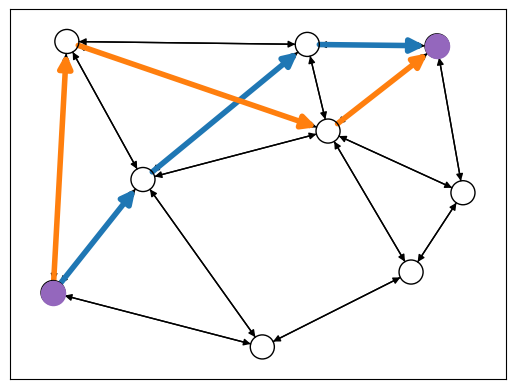
\includegraphics[width=\textwidth]{user0_with_protection.png}
  \end{subfigure}
  \begin{subfigure}[t]{0.33\textwidth}
    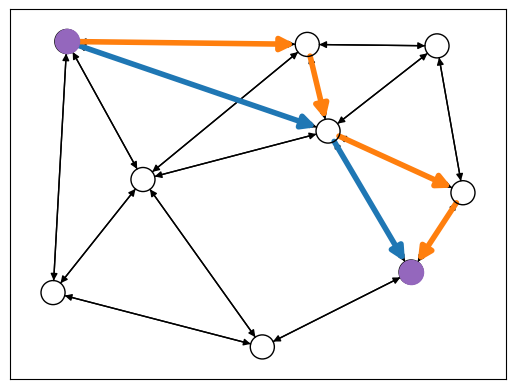
\includegraphics[width=\textwidth]{user1_with_protection.png}
  \end{subfigure}
  \begin{subfigure}[t]{0.33\textwidth}
    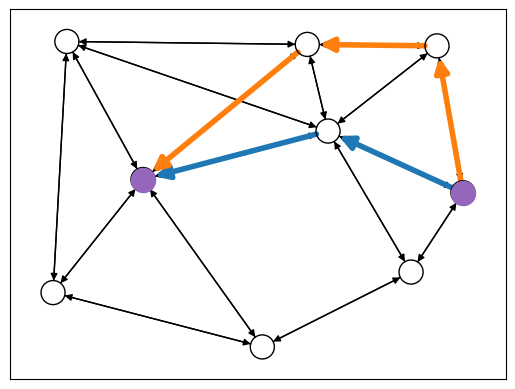
\includegraphics[width=\textwidth]{user2_with_protection.png}
  \end{subfigure}
  \caption{
    Egy hálózaton három felhasználó küld egyszerre adatot.
    Forrásuk és céljuk lilával, fő útvonaluk kékkel, mellék útvonaluk narancssárgával jelölve.
    Az élek súlya a csúcsok közötti távolság.
  } \label{fig:2.1}
\end{figure}

\subsection{Egyszerűsített 5G hálózat modellezése}
\label{sec:5gnetwork}

Az 5G hálózat egy egyszerűsített modellje látható a \ref{fig:2.2} ábrán.
A mobil eszközök (UE) a gNodeB állomásokra csatlakoznak.
A gNodeB-k és az átjáró közötti útvonalakat (a maghálózat további elemeit) egy-egy kapcsolat reprezentálja.
A modell csak a felmenő kapcsolatokat tartalmazza.
Mivel a gNodeB-k egymás között nem közvetítenek felhasználói adatforgalmat,\footnote{
  Bár az Xn protokoll lehetővé teszi, hogy a gNodeB-k közvetlenül kommunikáljanak, ez handover lebonyolítására és diagnosztikai adatok továbbítására használatos.
}
feltételezhető hogy minden UE forgalmának a célja az átjáró.

\usetikzlibrary{arrows.meta}
\begin{figure}[h]
  \centering
  \begin{tikzpicture}
    % Nodes
    \node[circle,minimum width=0.5cm,draw,label={UE$_1$}] (ue1) at (0,4) {};
    \node[circle,minimum width=0.5cm,draw,label={UE$_2$}] (ue2) at (0,2) {};
    \node[circle,minimum width=0.5cm,draw,label={UE$_3$}] (ue3) at (0,0) {};

    \node[circle,minimum width=0.5cm,draw,label={gNodeB$_1$}] (gb1) at (3,3.5) {};
    \node[circle,minimum width=0.5cm,draw,label=below:{gNodeB$_2$}] (gb2) at (3,.5) {};

    \node[circle,minimum width=0.5cm,draw,label=right:{gateway}] (gw) at (6,2) {};

    \draw[-{Stealth[scale=1.5pt]}] (ue1) -- (gb1);
    \draw[-{Stealth[scale=1.5pt]}] (ue1) -- (gb2);

    \draw[-{Stealth[scale=1.5pt]}] (ue2) -- (gb1);
    \draw[-{Stealth[scale=1.5pt]}] (ue2) -- (gb2);

    \draw[-{Stealth[scale=1.5pt]}] (ue3) -- (gb1);
    \draw[-{Stealth[scale=1.5pt]}] (ue3) -- (gb2);

    \draw[-{Stealth[scale=1.5pt]}] (gb1) -- (gw);
    \draw[-{Stealth[scale=1.5pt]}] (gb2) -- (gw);
  
    % Edges
  \end{tikzpicture}
  \caption{Az egyszerűsített 5G hálózatot ábrázoló gráf.} \label{fig:2.2}
\end{figure}

A mobil eszközök és állomások között vezeték nélküli a kapcsolat,
ezért a pozíciójuk hasznos információ.
Legyen a $v \in V \quad p(v)$ az adott csomópont pozíciója a térben.
Ekkor a mobil eszköz és állomás közötti kapcsolat súlya megadható a köztük lévő távolság
és $B$ alap feldolgozási idő összegeként.
Az állomás és az átjáró közötti kapcsolatok súlya beállítható az adott maghálózat valós felépítéséből kiindulva.
Így \eqref{eq:2.6} a teljes súlyfüggvény.
$U \subset V, N \subset V, gw \in V$ a mobil eszköz és állomás csúcsok halmazai, valamint az átjáró csúcsa.

\begin{equation}
  \forall e = (v_i, v_j) \in E \quad w(e) = \begin{cases}
    \vert p(v_i) - p(v_j) \vert + B, & \text{ha $v_i$ egy mobil eszköz} \\
    W_i, & \text{különben ($v_i$ egy állomás)}
  \end{cases} \label{eq:2.6}
\end{equation}

A többszörös csatlakozás, és több utas protokollok támogatása érdekében a modellt úgy kell módosítani,
hogy egy mobil eszköz akárhány részre tudja osztani a forgalmát.
Az $x_u(e), y_u(e)$ függvények értéktartománya tehát legyen a pozitív valós számok halmaza, és jelöljék azt,
hogy az adott élen a mobil eszköz mennyi fő és védelmi forgalmat küld.
A folyammegmaradási kényszer felírható a bázisállomásokra a \eqref{eq:2.7a} egyenlettel.
Mivel a gNodeB-átjáró kapcsolatok folyamait determinálják a gNodeB-be befutó folyamok,
ezért ezekre az élekre nem szükséges döntési változót felvenni.
A mobil eszközökből kifolyó fő forgalomnak pedig egyenlőnek kell lennie a felhasználó igényével,
ezt fejezi ki a \eqref{eq:2.7b} kényszer.

\begin{subequations}
  \begin{equation}
    \forall n \in N, \, e_{n} = (n, gw) \quad
    x_n(e_n) = \sum_{e=(u,n)}^{\inedge{n}} x_u(e) \,; \quad
    y_n(e_n) = \sum_{e=(u,n)}^{\inedge{n}} y_u(e) \label{eq:2.7a}
  \end{equation}
  \begin{equation}
    \forall u \in U \quad \sum_{e}^{\outedge{u}} x_u(e) = D_u \label{eq:2.7b}
  \end{equation}
\end{subequations}

Mivel az adatfolyam megosztott, nem szükséges, hogy a védelmi folyam éldiszjunkt legyen a fő folyammal.
Egy mobil eszköz például dönthet úgy, hogy több útvonalat tart fönn, és mindegyiken fő és védelmi forgalmat is számol.
Ez nem probléma, ha egy útvonal kiesése esetén a többin a védelmek és fő folyamok összege legalább akkora, mint a felhasználó forgalom igénye.
Hogy ez teljesüljön, felírható a \eqref{eq:2.8} kényszer.

\begin{equation}
  \forall u \in U \quad \forall e' \in \outedge{u} \quad
  E' = \outedge{u} \setminus \lbrace e' \rbrace, \quad
  \sum_{e}^{E'} x_u(e) + y_u(e) \geq D_u \label{eq:2.8}
\end{equation}

Az alulról korlátozó kényszerek ezzel készen vannak. A felső korlátot ismét az élek maximum kapacitása adja.
Az $x_u(e)$ és $y_u(e)$ függvények most önmagukban megadják az élen futó összes forgalmat,
így a kapacitás kényszer \eqref{eq:2.9}.

\begin{equation}
  \forall e \in E \quad \sum_{u}^{U} x_u(e) + y_u(e) \leq c(e) \label{eq:2.9}
\end{equation}

Végezetül a \eqref{eq:2.5} kifejezés ebben az esetben is használható célfüggvényként.

\newpage

A modell segítségével a hálózati eszközök viselkedése megfigyelhető telített és telítetlen hálózaton.\footnote{
  Egy telített hálózat olyan, amelynek kapcsolatainak kapacitása majdnem teljes kihasználtságú,
  több forgalmat a hálózaton nem lehet átvinni.
}
Legyen egy teszthálózatban olyan, amiben négyszer négyes mátrixban helyezkednek el állomások,
húsz mobil eszköz csatlakozik a hálózatra véletlenszerű pozícióval.
Mindegyik eszköz mindegyik állomásra csatlakozik.
Kezdetben az állomás-átjáró élek kapacitása legyen elég nagy, hogy a felhasználók igényeit gond nélkül elszállítsa a hálózat,
aztán csökkenjenek addig, amíg a hálózat telített nem lesz.
Minden egész kapacitás értékre futtatva a szoftvert,
a kapott eredményt a \ref{fig:2.3} és \ref{fig:2.4} ábrán láthatók.

A \ref{fig:2.3a} ábra a mobil eszközök összes kapcsolatát mutatja az egyes kapacitásszinteken.
Egy mobil eszköz eredetileg minden állomáshoz kapcsolódik, de azok a kapcsolatok,
amiken sem fő, sem védelmi folyamot nem számol, felbonthatók.
Az ábrán az ez után maradt kapcsolatok jelennek meg. Eleinte a mobil eszközök a hozzájuk legközelebb eső, így legkisebb súlyú kapcsolatokon küldik minden adatukat,
így kevés kapcsolatot tartanak fent.
A kapacitás csökkenése miatt azonban a hálózat telített lesz.
Az összfolyamot, tehát a fő és védelmi folyam összegét a hálózat már nem lesz képes elszállítani.
Mivel a felhasználók igénye adott, csak a védelmi folyam csökkenthető.
Látható, hogy a mobil eszközök egyre több kapcsolatot tartanak fönn,
hiszen ekkor egy kapcsolatra a teljes folyam igény kisebb része jut,
így egy él kiesése esetén kevesebb forgalmat kell másfelé irányítani,
tehát összesen kevesebb védelmet kell biztosítani.
A védelmi forgalom csökkenése látható a \ref{fig:2.3b} ábrán.
A védelmen spórolva már elszállítható minden adat a hálózaton.

\begin{figure}[h]
  \begin{subfigure}[t]{0.5\textwidth}
    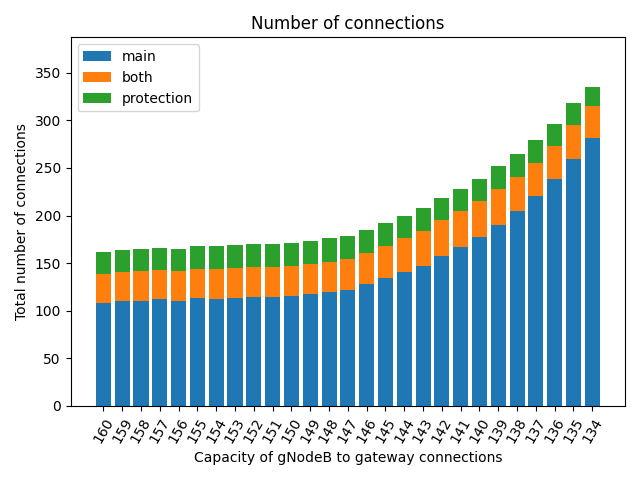
\includegraphics[width=\textwidth]{number_of_connections.png}
    \caption{
      A mobil eszközök összes fenntartott kapcsolata az egyes kapacitás értékekre.
    } \label{fig:2.3a}
  \end{subfigure}
  \begin{subfigure}[t]{0.5\textwidth}
    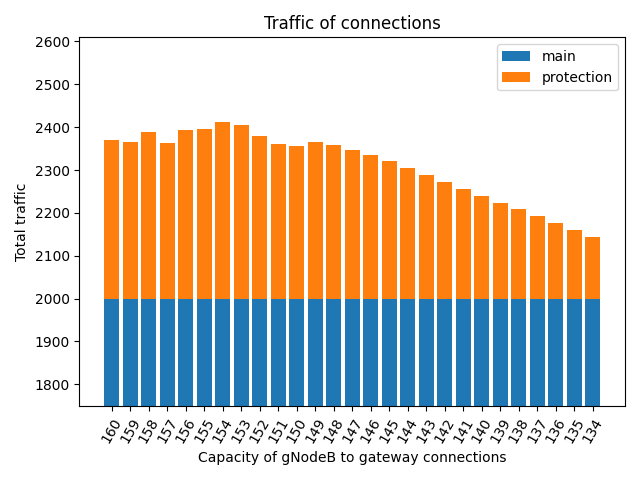
\includegraphics[width=\textwidth]{traffic_of_connections.png}
    \caption{
      A mobil eszközök által generált összforgalom.
    } \label{fig:2.3b}
  \end{subfigure}
  \caption{Eszközök kapcsolatszámának növekedése, a védelmen való spórolás céljából.}
  \label{fig:2.3}
\end{figure}

Ez addig folytatható, amíg már az összes mobil eszköz az összes állomásra csatlakozik.
Ez után a kapcsolatok száma nem növelhető, ezért kisebb kapacitáson a védelem nem biztosítható.
A \ref{2.4a} ábra mutatja a mobil eszközök kapcsolatszámának eloszlását.
Itt is megfigyelhető, hogy az eszközök egyre több kapcsolatot létesítenek a védelem csökkentése érdekében.
A teszthálózatban a minimális kapacitás érték százharmincnégy,
ekkor már majdnem mindegyik eszköz mind a tizenhat állomásra csatlakozik.
A \ref{2.4b} ábrán négy specifikus kapacitás értékre látható a kapcsolatszámok konkrét eloszlása.

\begin{figure}[h]
  \begin{subfigure}[t]{0.5\textwidth}
    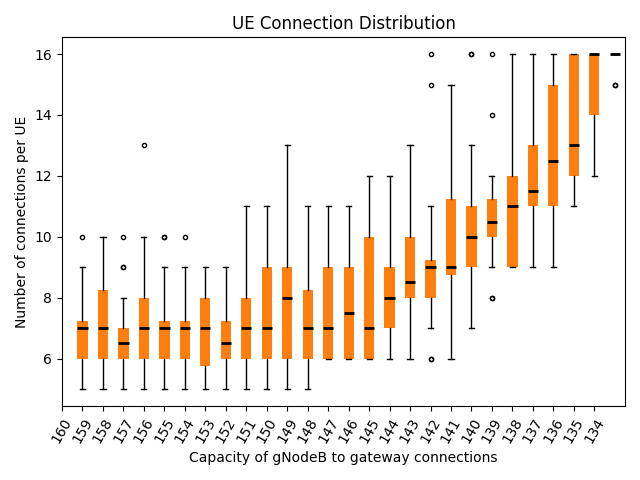
\includegraphics[width=\textwidth]{ue_connection_distribution.png}
    \caption{
      A mobil eszközök által fenntartott kapcsolatok számának eloszlása.
    } \label{fig:2.3a}
  \end{subfigure}
  \begin{subfigure}[t]{0.5\textwidth}
    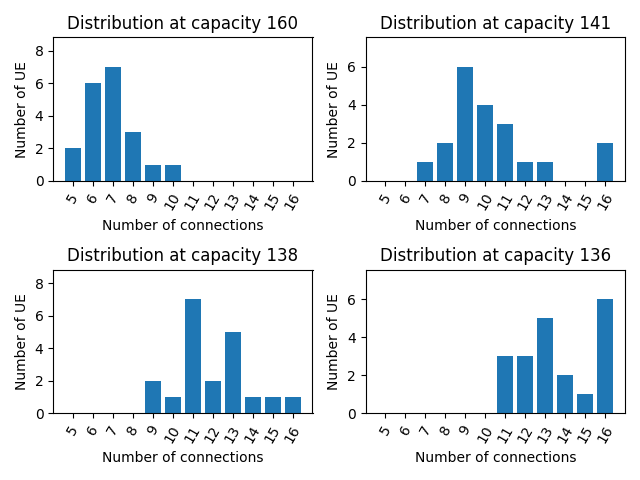
\includegraphics[width=\textwidth]{specific_distribution.png}
    \caption{
      A konkrét kapcsolatszám eloszlás néhány specifikus kapacitáson.
    } \label{fig:2.3b}
  \end{subfigure}
  \caption{A kapcsolatszámok eloszlásának alakulása.}
  \label{fig:2.4}
\end{figure}

\newpage

\subsection{Összefoglalás}
\label{sec:osszefoglalas}

Egy hálózat komponenseire és kapcsolataira lineáris kényszerek, és lineáris célfüggvény adható.
Ezek alapján az optimális hálózati folyam meghatározása egy lineáris programozási probléma.
A hálózati szolgáltatás minőségének javítására a fő adatforgalom mellé
védelmi adatforgalom számolható, amivel egy kapcsolat kiesése esetén a kommunikáció zavartalanul folytatódhat.
A modell kiterjeszthető, hogy támogassa a többszörös csatlakoztatást.
Egy egyszerűsített 5G hálózaton elvégzett teszten látható, hogy a modell hogyan használható
a hálózati eszközök kapcsolatszámának, védelmi folyamának meghatározására az optimális
hálózati folyam elérése érdekében.
 
%==================================================================
\section{Irodalom, és csatlakozó dokumentumok jegyzéke}
\label{sec:irod-es-csatl}

\begin{thebibliography}{9}
\label{sec:tanulm-irod-jegyz}

\bibitem{multiconnectivity} S. A. Busari, R. Mumtaz and J. Gonzalez,
\emph{MULTI-CONNECTIVITY IN 5G NEW RADIO STANDARDS},
2020. november 30.
Elérhető: \url{https://www.standardsuniversity.org/e-magazine/december-2020/multi-connectivity-in-5g-new-radio-standards/}
2023. november 24-én

\bibitem{mptcp} Olivier Bonaventure, Mark Handley, Costin Raiciu,
\emph{An Overview of Multipath TCP}
2012. október
Elérhető: \url{https://www.usenix.org/system/files/login/articles/login1210_bonaventure.pdf}
2023. november 24-én

\end{thebibliography}

%==================================================================
\subsection{A csatlakozó dokumentumok jegyzéke}
\label{sec:csat-irod}

Az elkészített program teljes forráskódja megtalálható az alábbi GitHub repository-ban:\\
\url{https://github.com/Kavefozogepezet/temalab-5g.git}

\end{document} 

%%% Local Variables: 
%%% mode: latex 
%%% TeX-master: t 
%%% End:

